\chapter{Traffic analysis}

\section{Data collection}

We used traffic of 4G cell towers traffic data to study self-similarity of the network.These cell towers serve user equipment in their vicinity. When a user makes a data service request, that device will be served by a 4G cell closest to the user. The traffic of a cell within an hour is given by the data capacity of all devices served by the station. 
\\Example: Cell X is serving 30 subscribers, assuming if a customer on average uses 20Mb per hour. Traffic of cell X that hour = 30 * 20 = 600Mb.\\\\
Data consists of 50 cells. Approximately the data is collected over 1 year x 24 hours x 57 cells.
We will see that the nature of traffic varies from time to time, there is peak traffic around 10-12 AM and 11-12PM, and low traffic is observed during early hours of the day.

\section{Traffic representation}

A sample real world LTE traffic data of one of the cells is represented below. The y-axis represents traffic accumulated at a eNode base station in Megabytes per hour over 1 year time frame.
\begin{figure}[H]
    \centering
    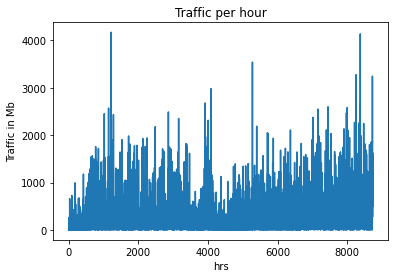
\includegraphics{traffic_per_hour.png}
    \caption{Traffic/hour}
    \label{fig:traffic_per_hour}
\end{figure}

Next, we aggregate the traffic accumulated per 10 hours by summing the 10 non-overlapping consecutive traffic per hour.
\begin{figure}[H]
    \centering
    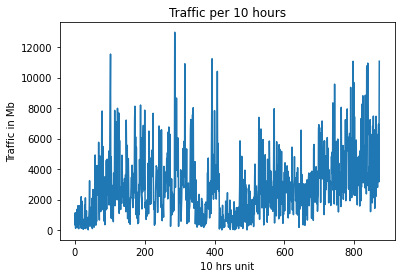
\includegraphics{traffic_per_10_hours.png}
    \caption{Traffic/10 hours}
    \label{fig:traffic_per_10_hour}
\end{figure}

\section{Variance-time plots}

For the data represented above, the $log(X^{m})$ vs $log(m)$ is plotted below,the blue cross points represent the log of variance of aggregated time series and the log of aggregation size, the red line represents a line with slope -1. We can clearly see that the points follow along a line with slope between 0 and -1.
\begin{figure}[H]
    \centering
    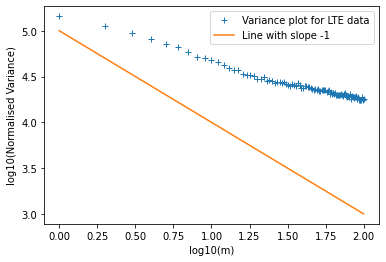
\includegraphics{Var plot.png}
    \caption{log Variance plot}
    \label{fig:traffic_per_10_hour}
\end{figure}

To calculate this slope we use linear regression to fit them along a line, The plotted curve is fitted with a Y=mX+C curve with best fit slope of -0.44535
 and y-intercept of 5.11624
 
 $\implies  -\beta = -0.44535 $
 $\implies H =1-\beta/2=1-(0.44535)/2=0.777325$
\begin{figure}[H]
    \centering
    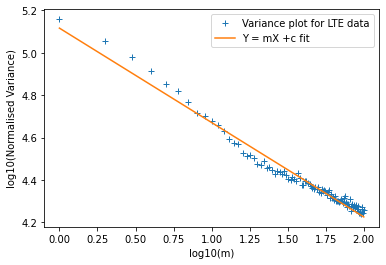
\includegraphics{line_fit.png}
    \caption{Fitting data on a straight line}
    \label{fig:line}
\end{figure}

We take data from more eNode base stations and verify the self-similarity of the traffic using the same method as above, the results of the fit and hurst-parameter are given below
\begin{figure}[H]
    \centering
    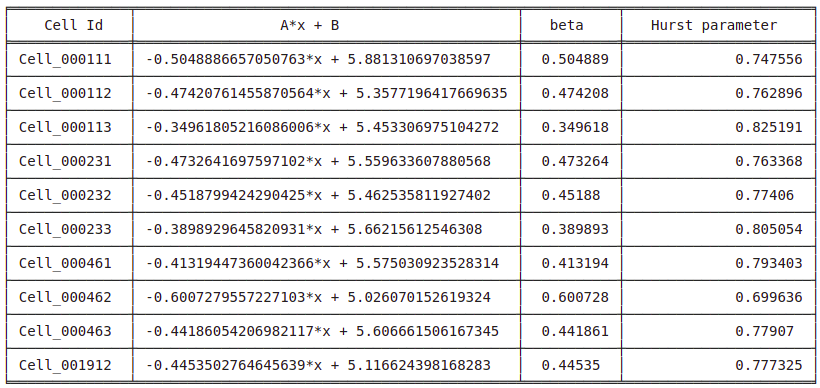
\includegraphics[scale =0.7]{table_H.png}
    \caption{Table of Hurst parameter for different cells}
    \label{fig:table}
\end{figure}



\section{Hourly traffic in a week}

Traffic of all hours in a week are averaged in the data and is plotted below

The data points start from Wednesday hour 0, and include traffic for each hour upto an year.
We can observe that the traffic in the early hours of the day is much less compared to the peak traffic observed within a day.

\begin{figure}[H]
    \centering
    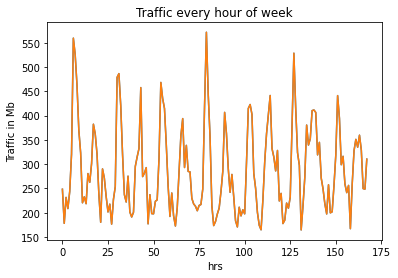
\includegraphics{everyhour.png}
    \caption{Traffic per hour in a week}
    \label{fig:everyhour}
\end{figure}

\section{Daily traffic in a week}
Traffic of all days in a week are averaged in the data and is plotted below

We can observe that the traffic is more during Wednesdays and Mondays, which is generally true for internet traffic as well.

\begin{figure}[H]
    \centering
    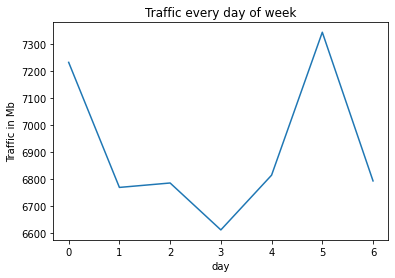
\includegraphics{everyday.png}
    \caption{Traffic per day in a week}
    \label{fig:everyday}
\end{figure}
